\documentclass{article}


\usepackage[margin=1in]{geometry}
\usepackage{amsmath}
\usepackage{graphicx}
\usepackage{tabu}
\usepackage{float}
\usepackage{listings}
\usepackage{color}
\usepackage{caption}


\lstdefinestyle{customc}{
    belowcaptionskip=1\baselineskip,
        breaklines=true,
          frame=L,
            xleftmargin=\parindent,
              language=C,
                showstringspaces=false,
                  basicstyle=\footnotesize\ttfamily,
                    keywordstyle=\bfseries\color{green!40!black},
                      commentstyle=\itshape\color{purple!40!black},
                        identifierstyle=\color{blue},
                          stringstyle=\color{orange},
                      }


\author{Zachary Vogel\quad James Pentz}
\title{Embedded Software Essentials Project 4\\ ECEN 5013}
\date{\today}

\begin{document}
\begin{titlepage}
    \centering
    \vspace*{2cm}
    {\scshape\Huge Embedded Software Essentials \par}
    \vspace{2cm}
    {\scshape\Large Project 4: SPI with External Peripherals and Code Abstraction \par}
    \vspace{2.5cm}
    {\Large \scshape Zachary Vogel \& James Pentz\par}
    \vspace{1cm}
    {\large \itshape Professor: Alexander Fosdick}
    \vfill
    {\large \today\par}
\end{titlepage}

\section*{Introduction}
In this project we are to explore the SPI capabilities of both the KL25Z freedom board and the Beaglebone Black as they interface with two Nordic transceiver SPI modules. In the first section of this project we will implement code that will initialize the SPI modules on both devices and write out and read from the Nordic device. Part 2 will focus on streaming data over the two transceivers to communicate from one to the other. The final section, which is extra credit will focus on
sending control data based on a structure of our own design from one device to another. All of the code as well as the report is on James Pentz's github repository at:\\

http://github.com/jgpentz/ecen5013\_projects

\section*{Project Procedure Results}
\subsection*{Part 1: Serial Peripheral Interface}
This section was about familiarizing ourselves with the different SPI interfaces and the nordic chips. Specifically, we wanted to make sure both of the devices could read to and write from both of the nordic chips.To accomplish this we began by writing a low level SPI driver on the freedom and a higher level nordic library that utilizes those SPI drivers. Since the SPI drivers already existed for the BeagleBone, all we did for that was write a nordic library. Ideally this high level
nordic library would be exactly the same for both the BeagleBone and the freedom board, but we didn't have time to implement this library so that it would work at either compile time or run time. Below is the required capture images showing we had data moving between the freedom board and the nordic chip. We had similar code functioning for the BeagleBone, but it was shifted left by 1 bit for some reason. This prevented any type of further communication because one has to send the correct bits
to the configuration register just to write and read from the chip.

\begin{figure}[H]
    \centering
    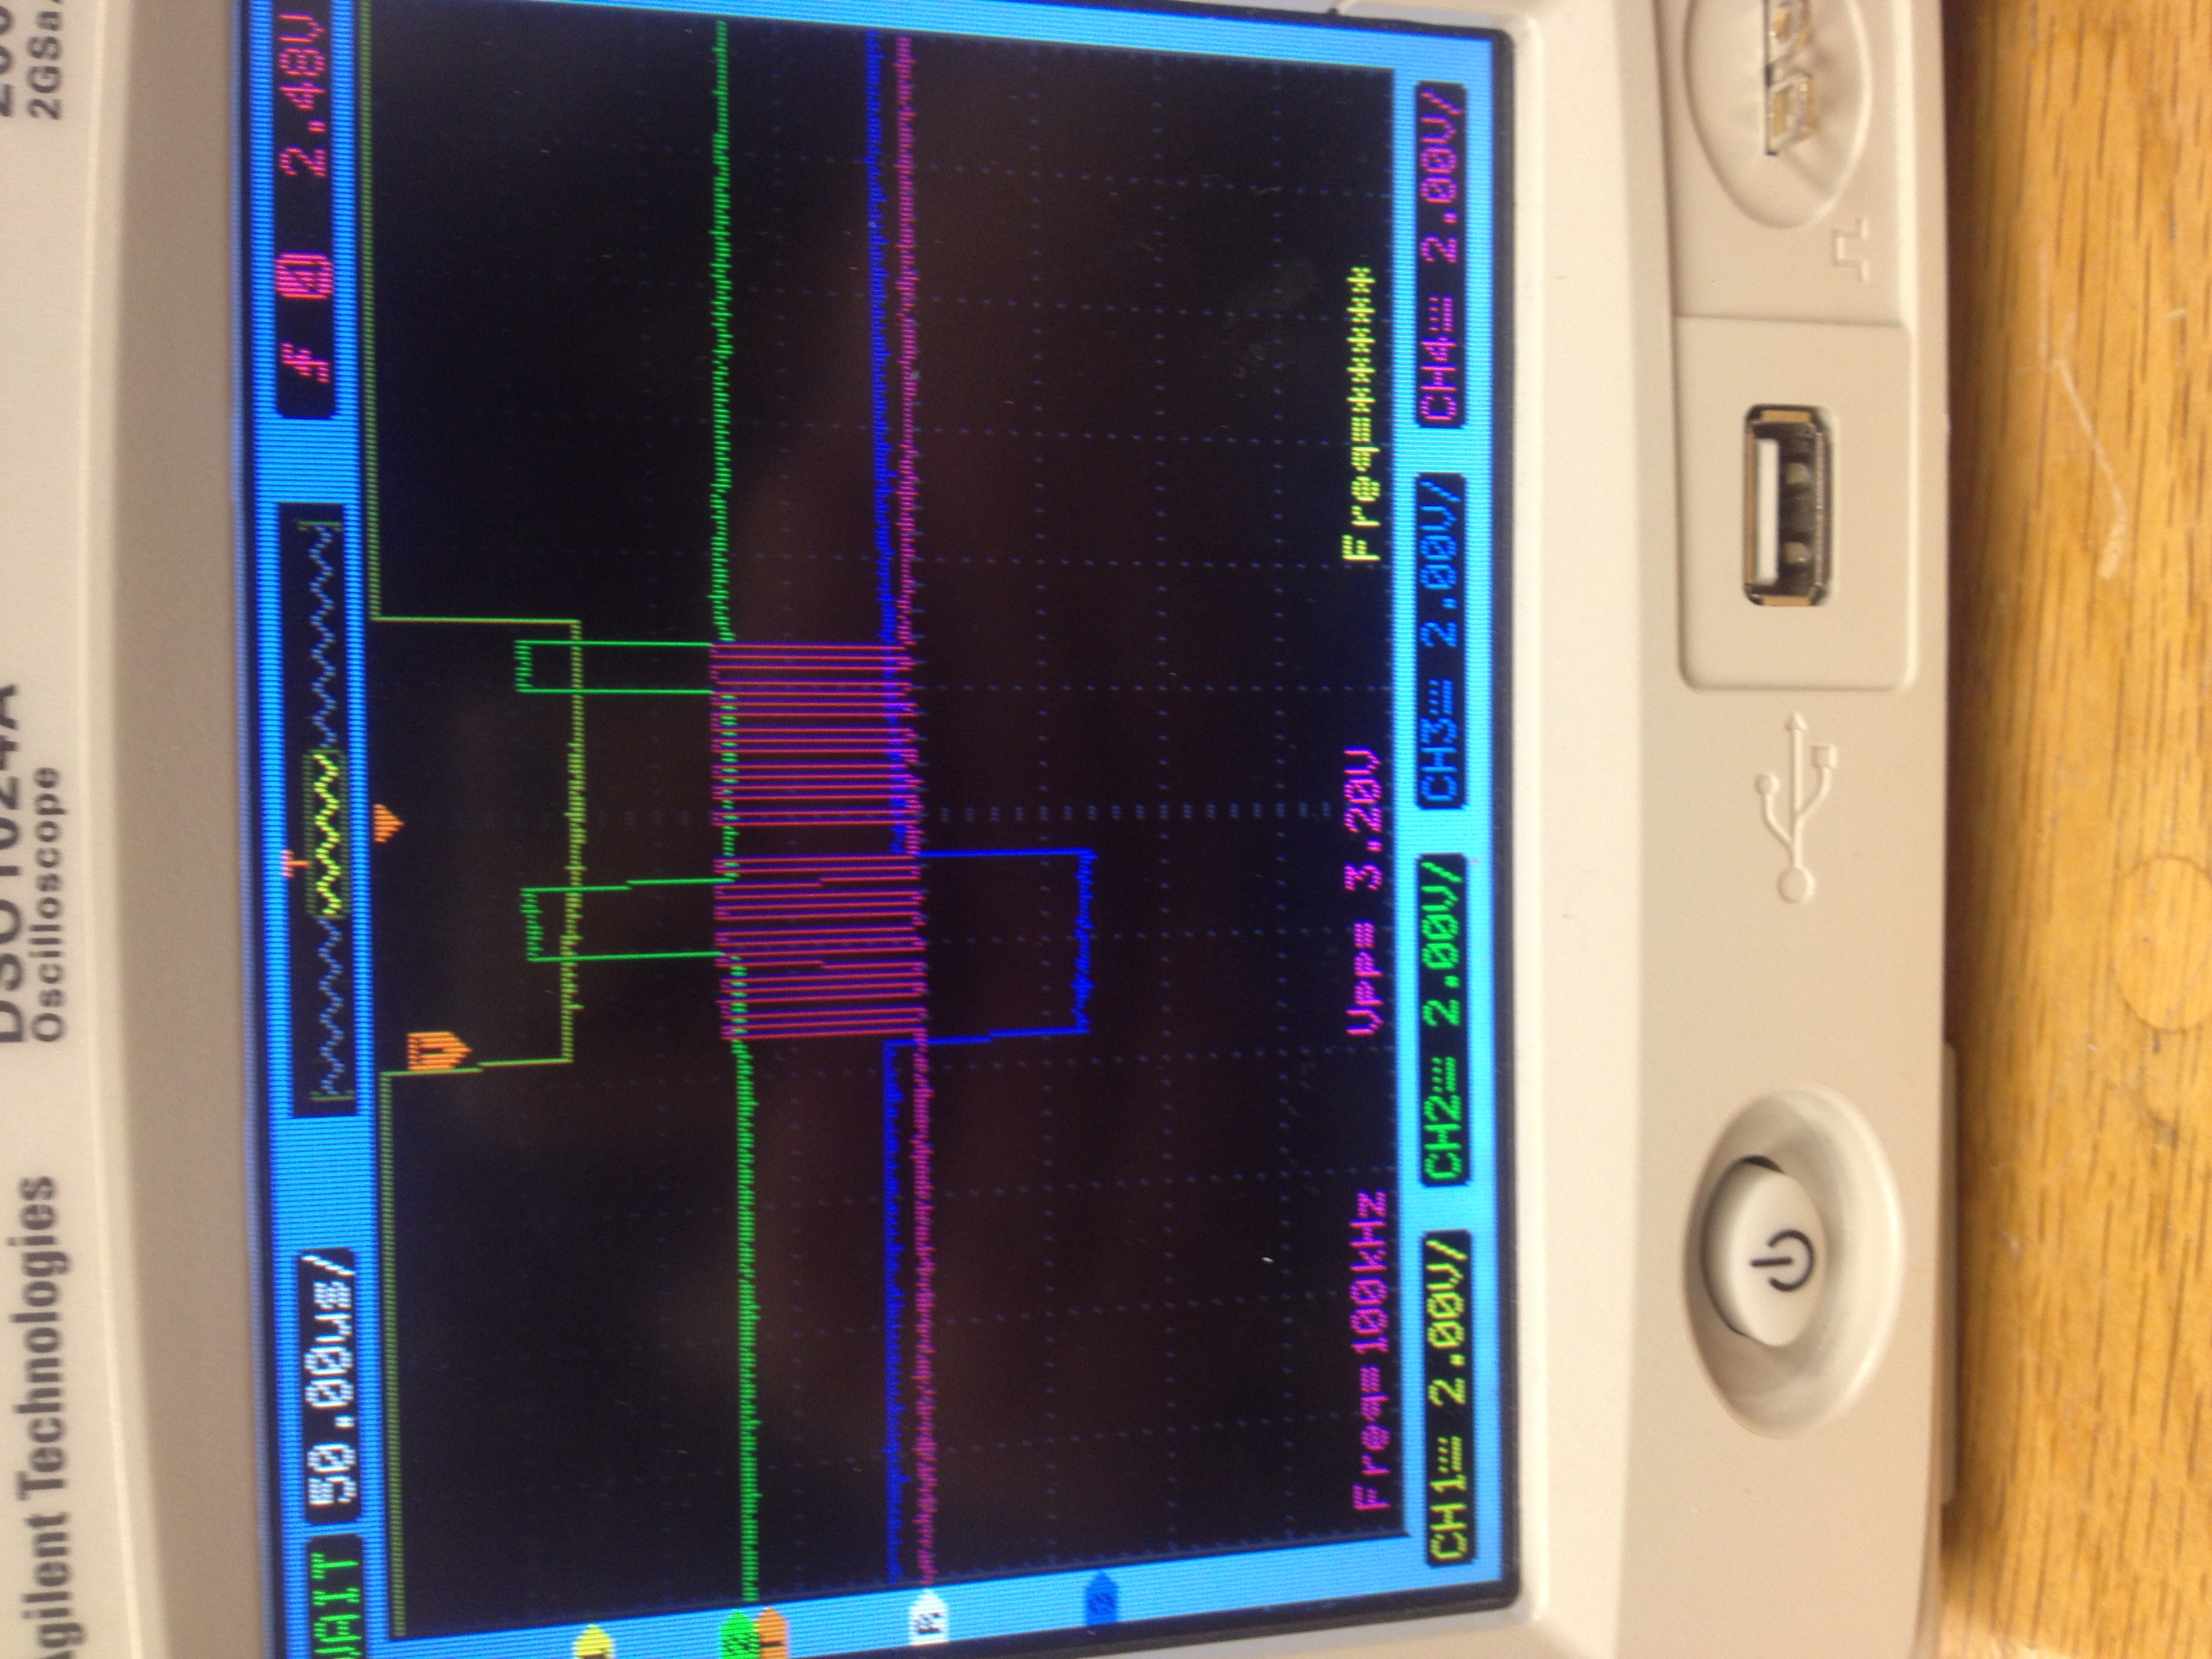
\includegraphics[width=0.6\textwidth,angle=-90]{config_read.jpg}
    \caption{Reading from the config register}
\end{figure}

\begin{figure}[H]
    \centering
    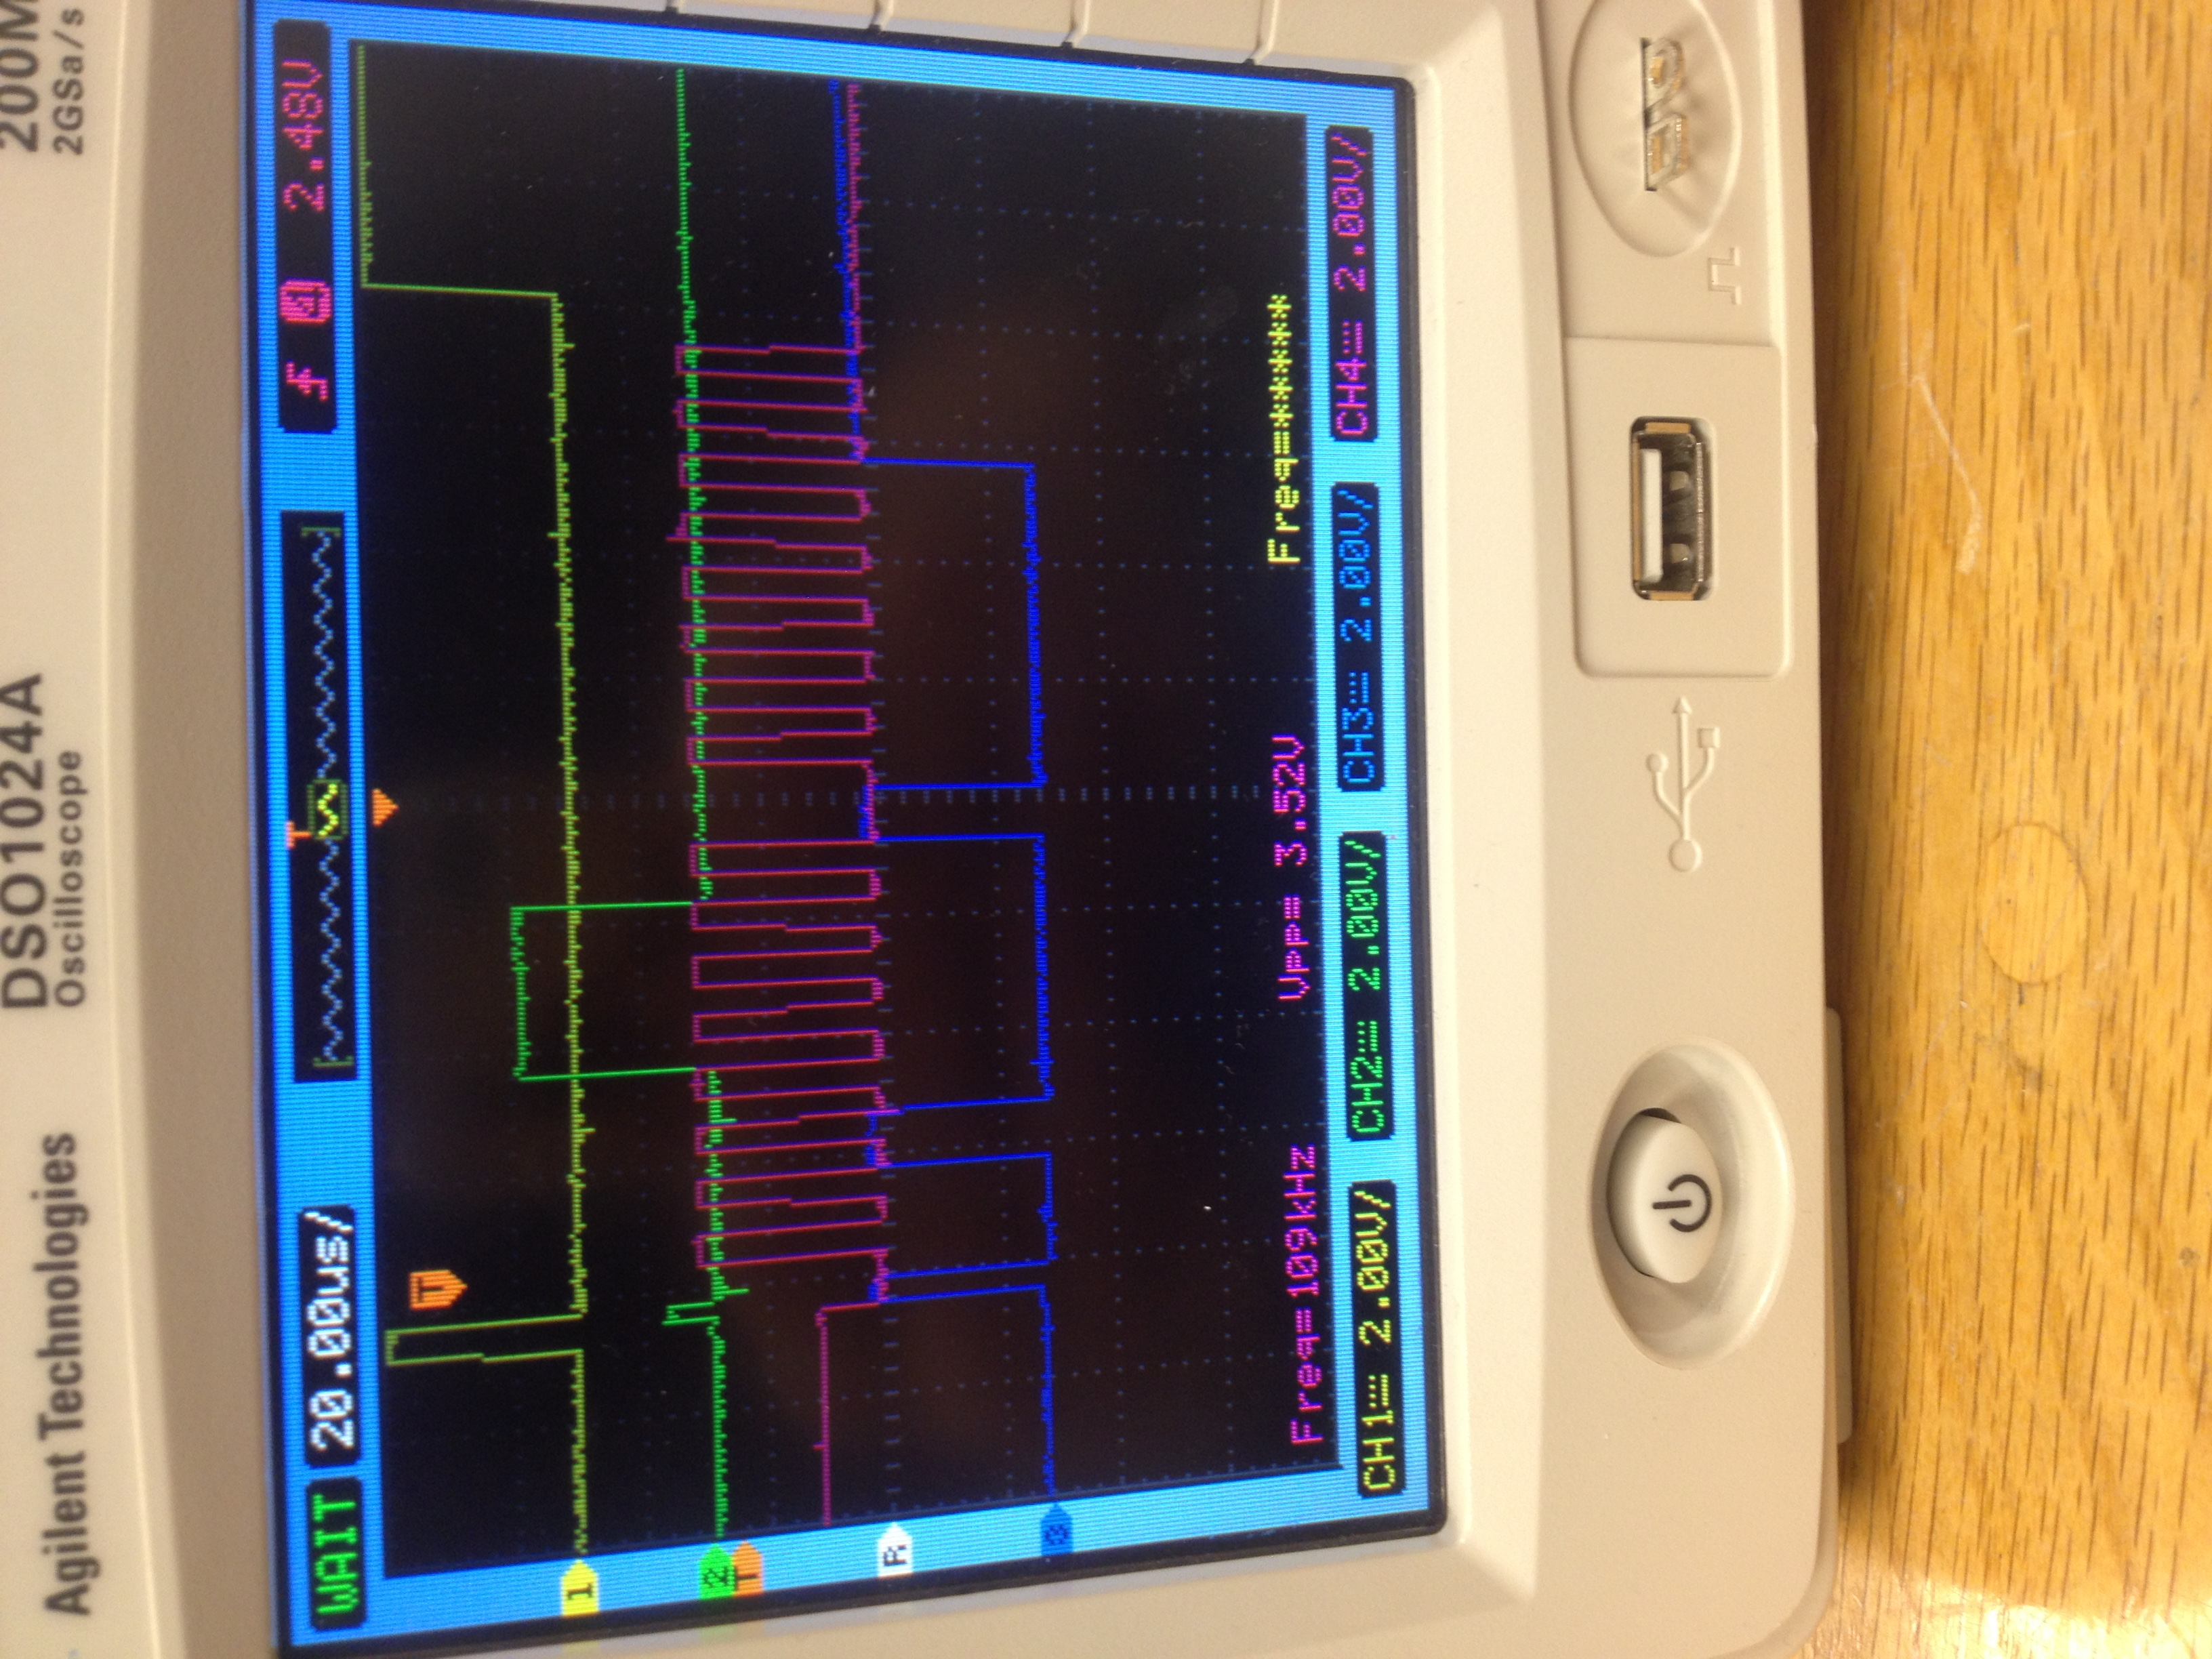
\includegraphics[width=0.6\textwidth,angle=-90]{config_write.jpg}
    \caption{Writing to the config register}
\end{figure}

\begin{figure}[H]
    \centering
    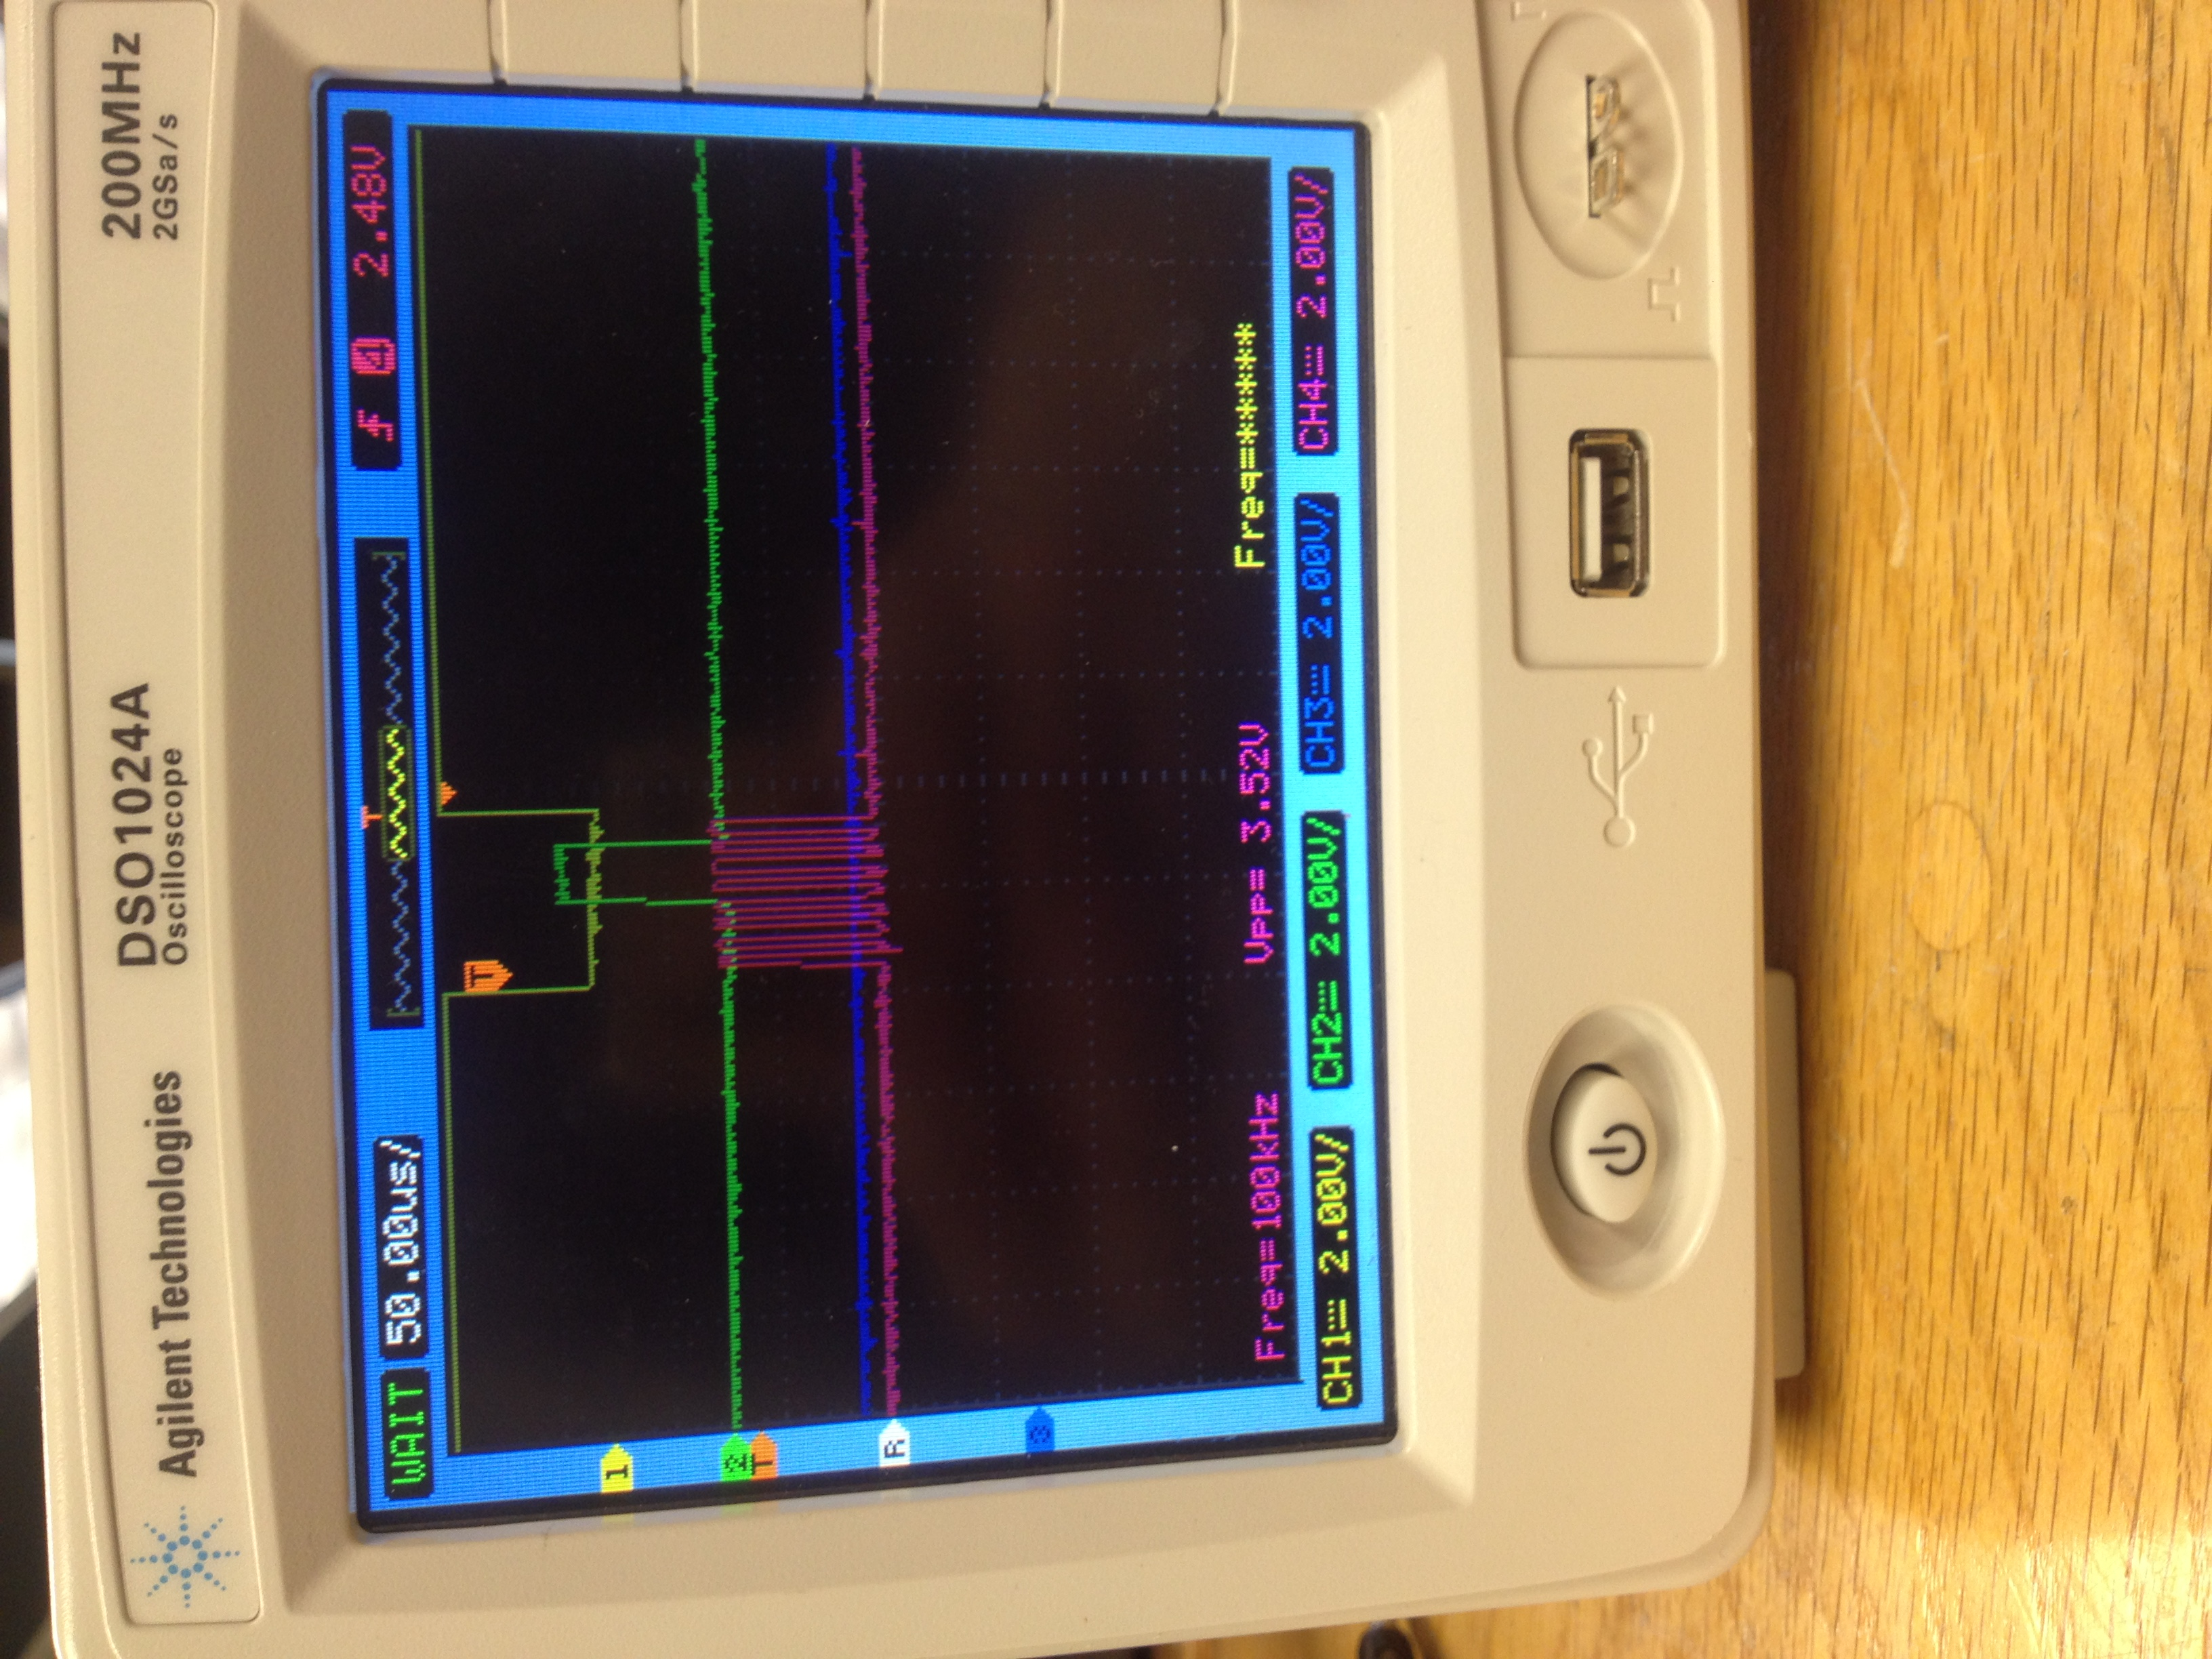
\includegraphics[width=0.6\textwidth,angle=-90]{status_read.jpg}
    \caption{Reading from the status register}
\end{figure}

\begin{figure}[H]
    \centering
    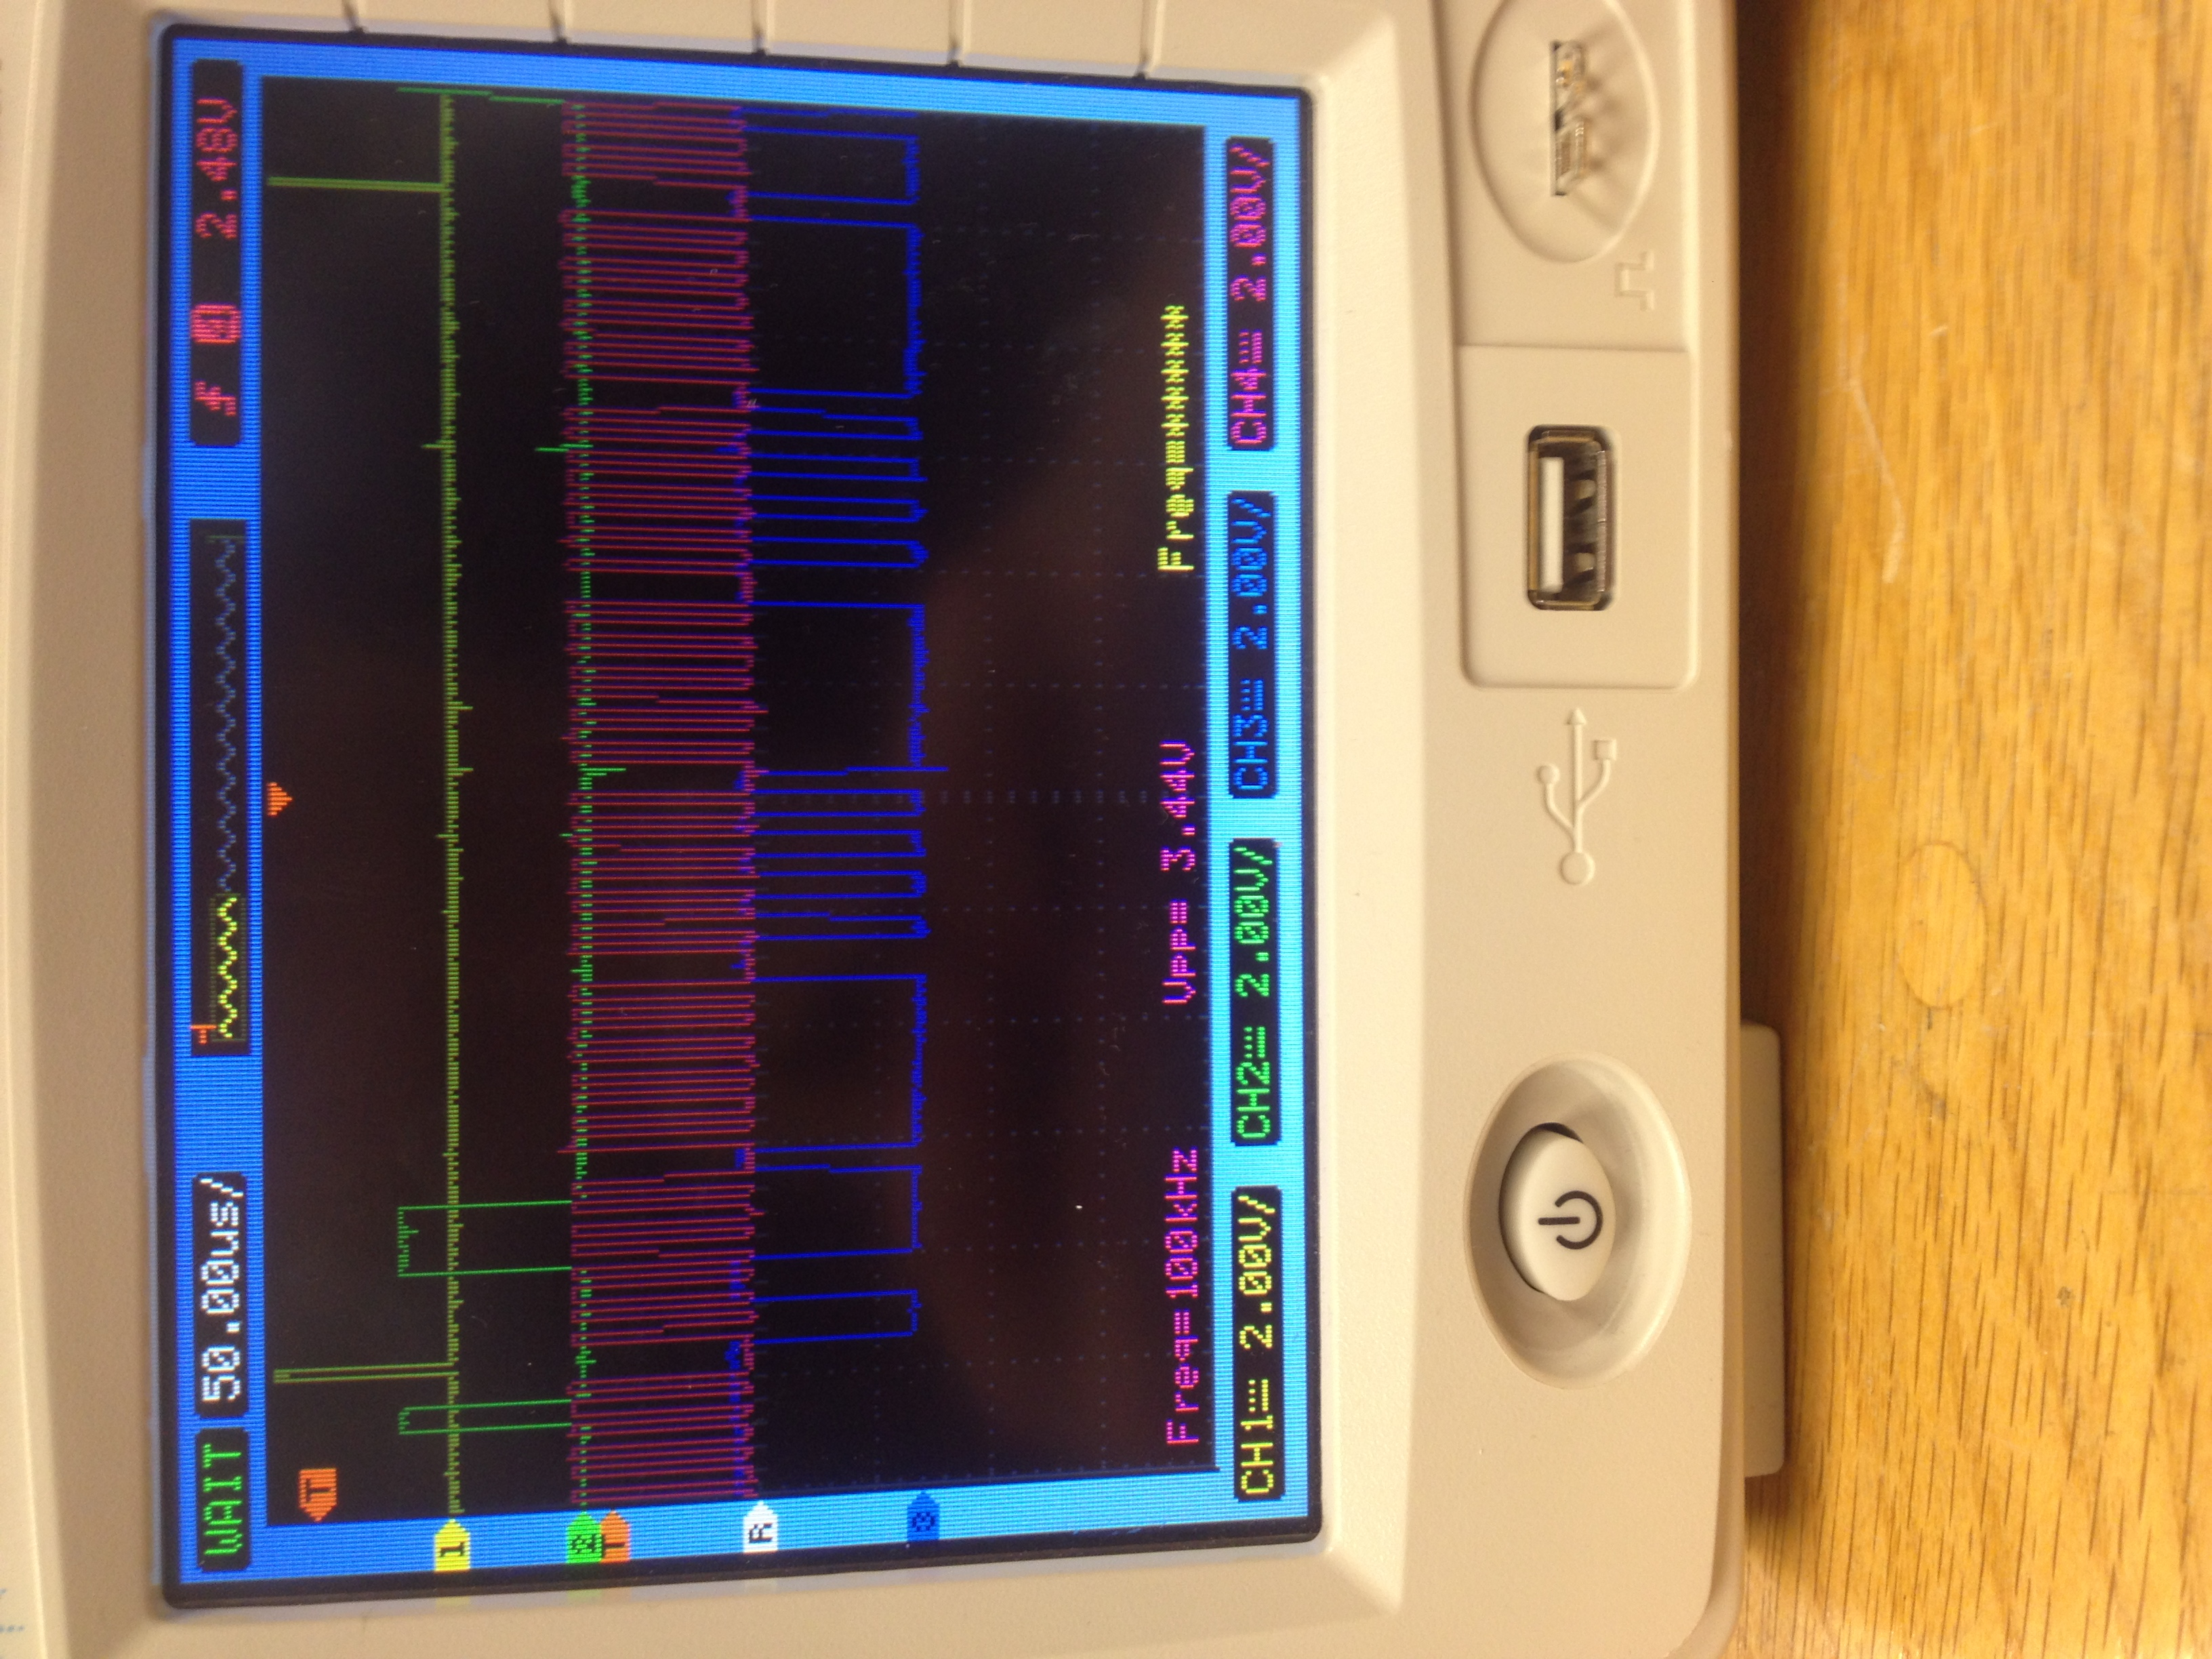
\includegraphics[width=0.6\textwidth,angle=-90]{tx_addr_write.jpg}
    \caption{Writing to the tx register}
\end{figure}

\begin{figure}[H]
    \centering
    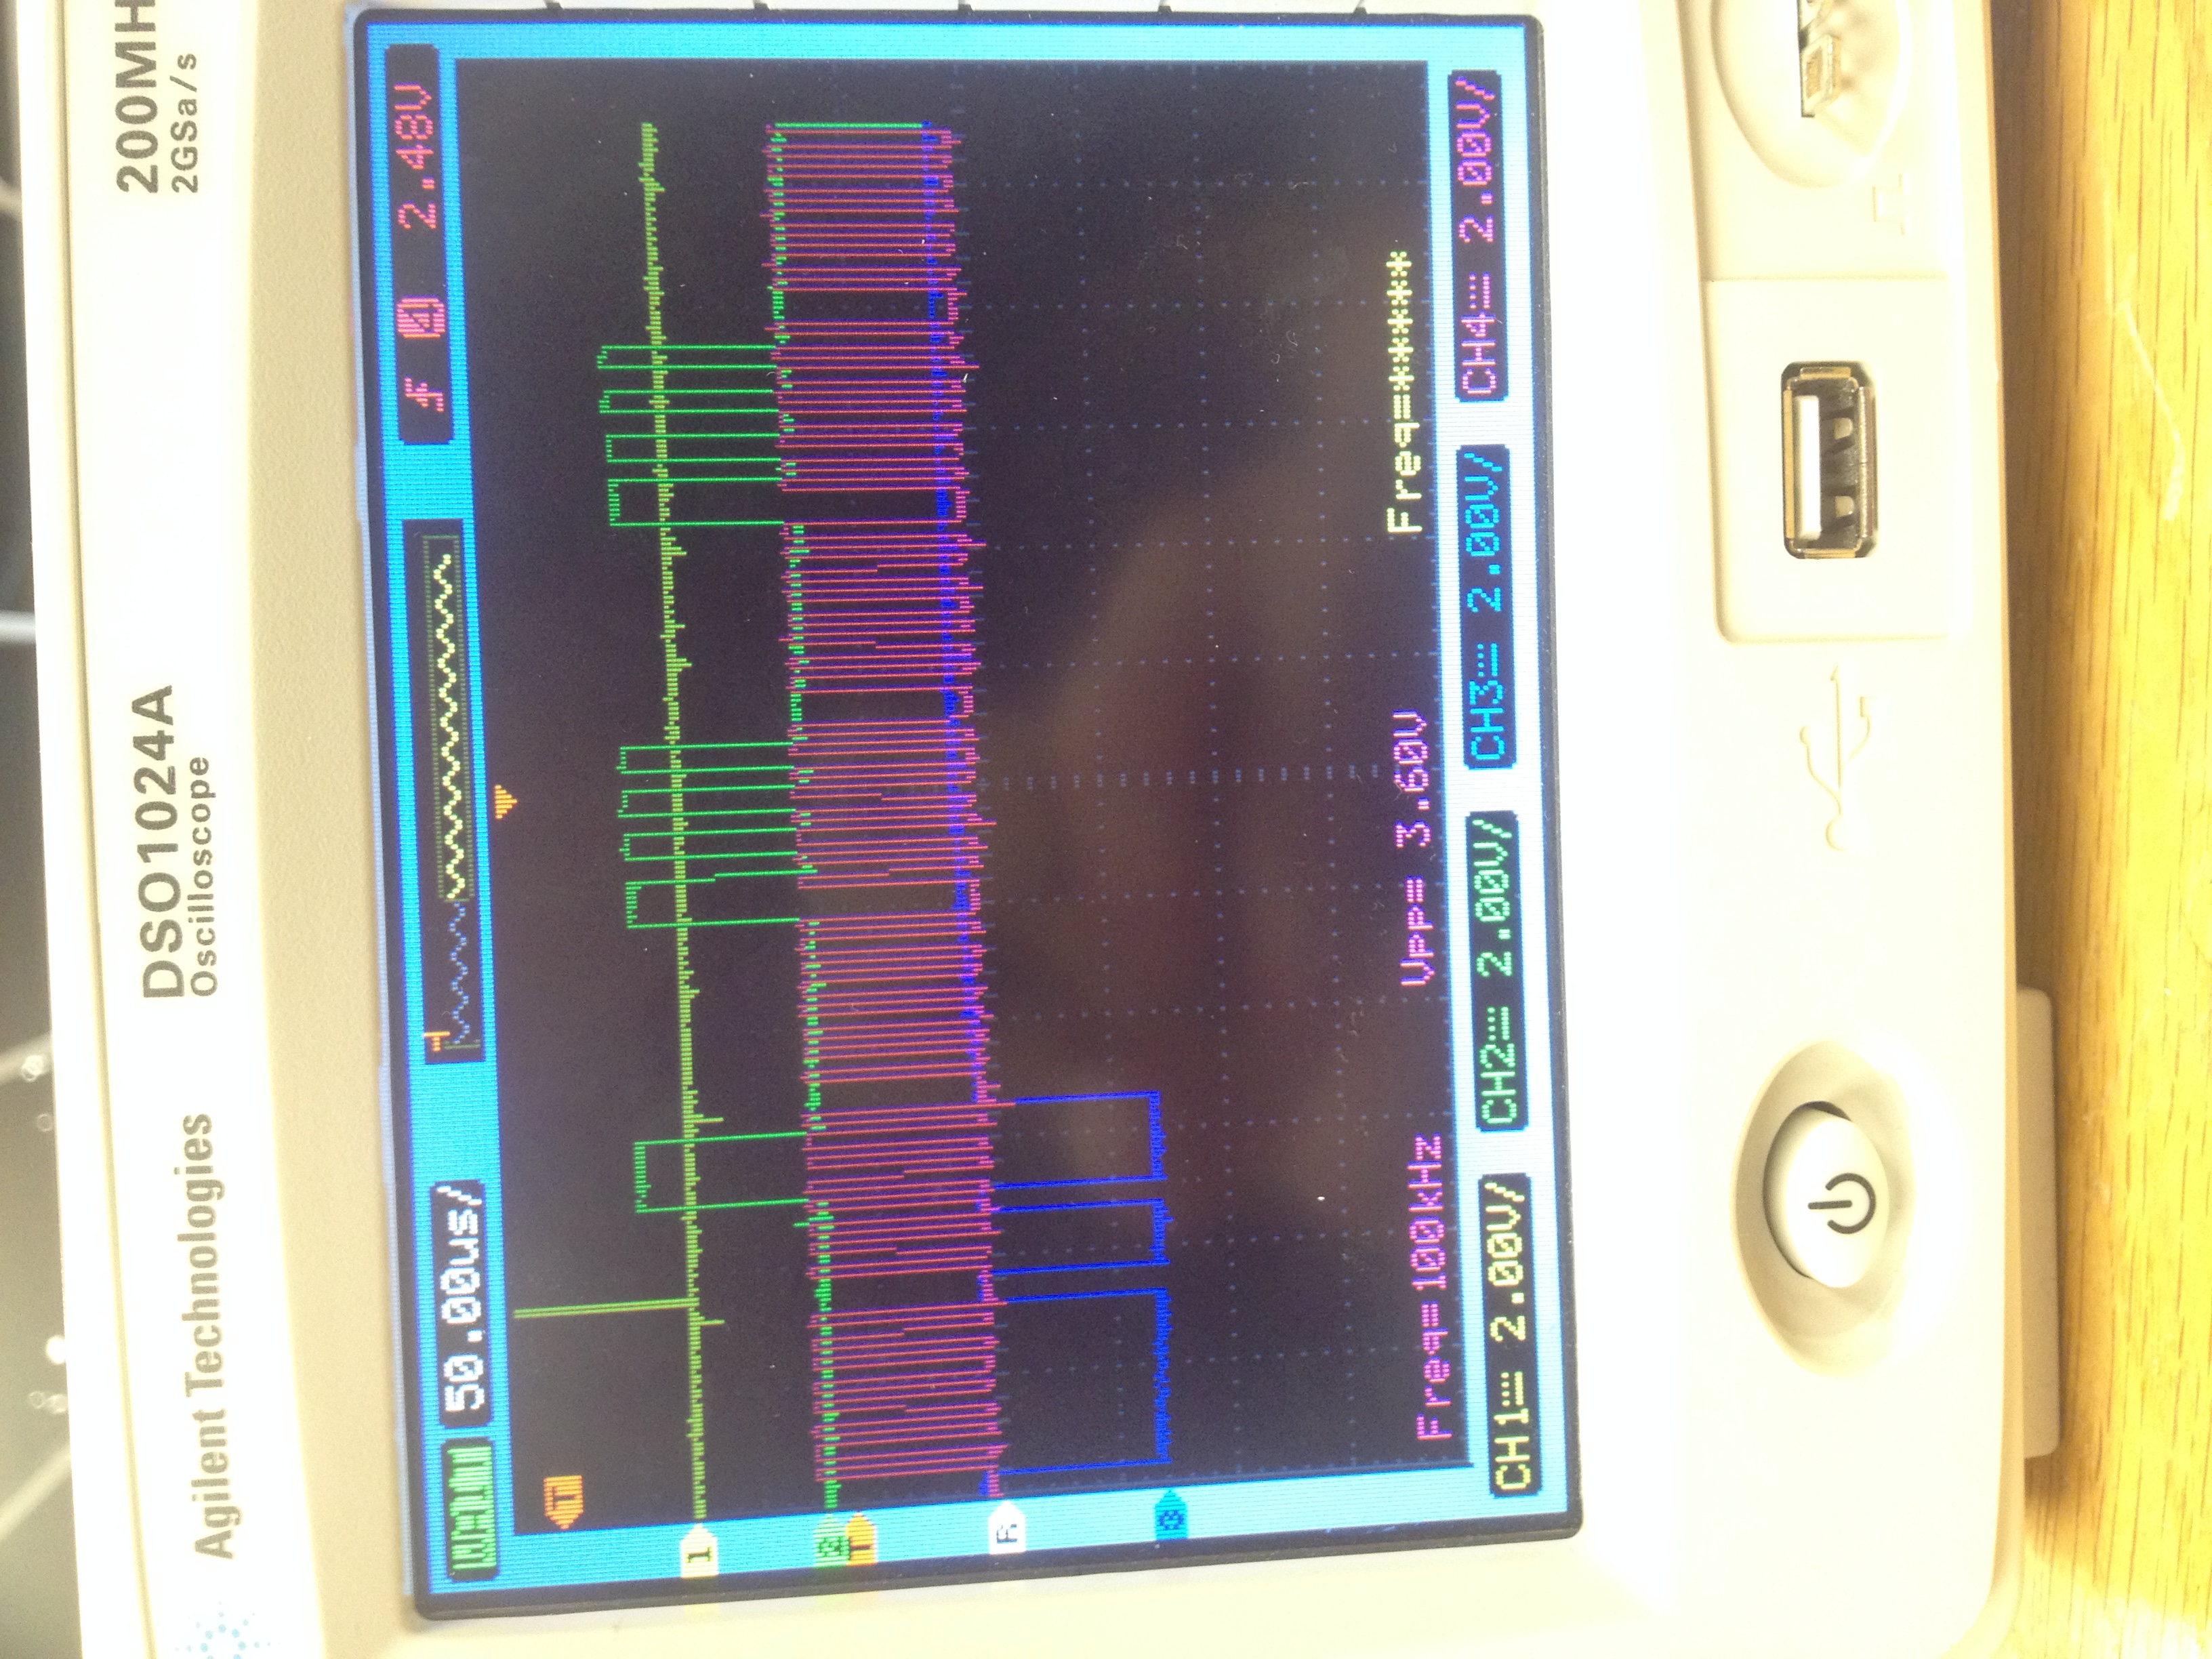
\includegraphics[width=0.6\textwidth,angle=-90]{tx_addr_read.jpg}
    \caption{Confirming that we wrote to the tx register by reading from it}
\end{figure}

\begin{figure}[H]
    \centering
    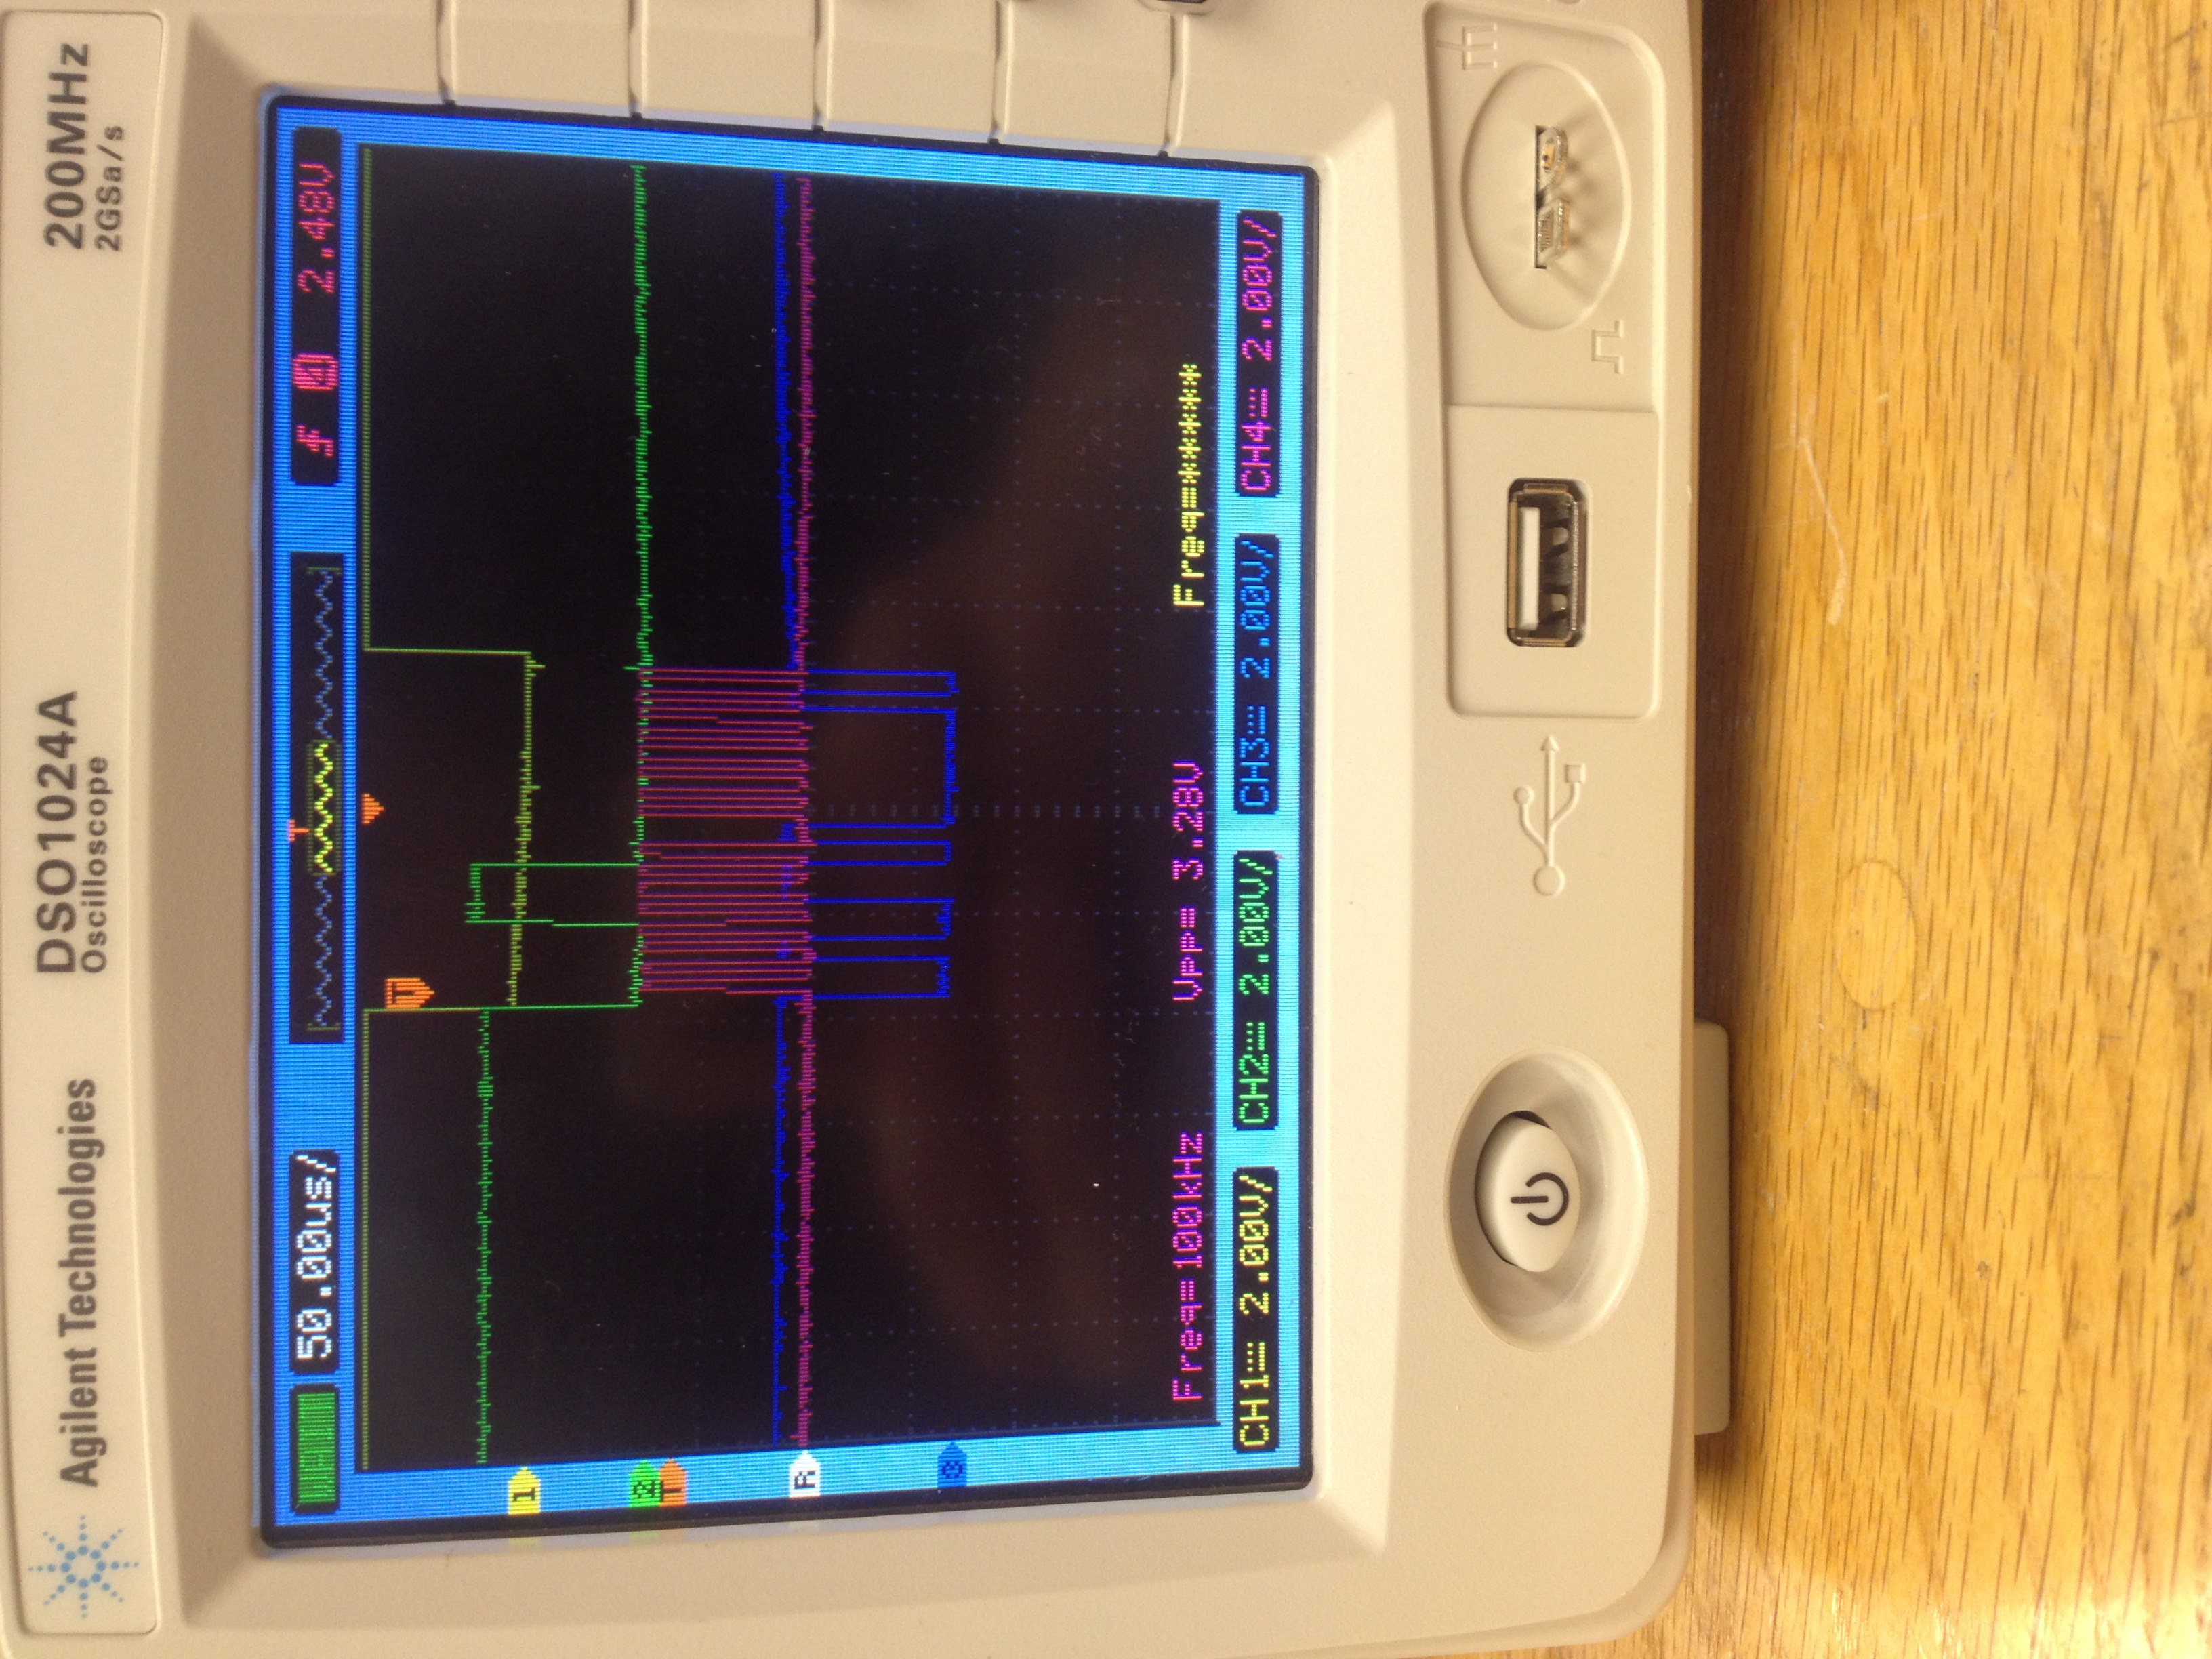
\includegraphics[width=0.6\textwidth,angle=-90]{pwr_config_write.jpg}
    \caption{Writing to the RF configuration register}
\end{figure}

\begin{figure}[H]
    \centering
    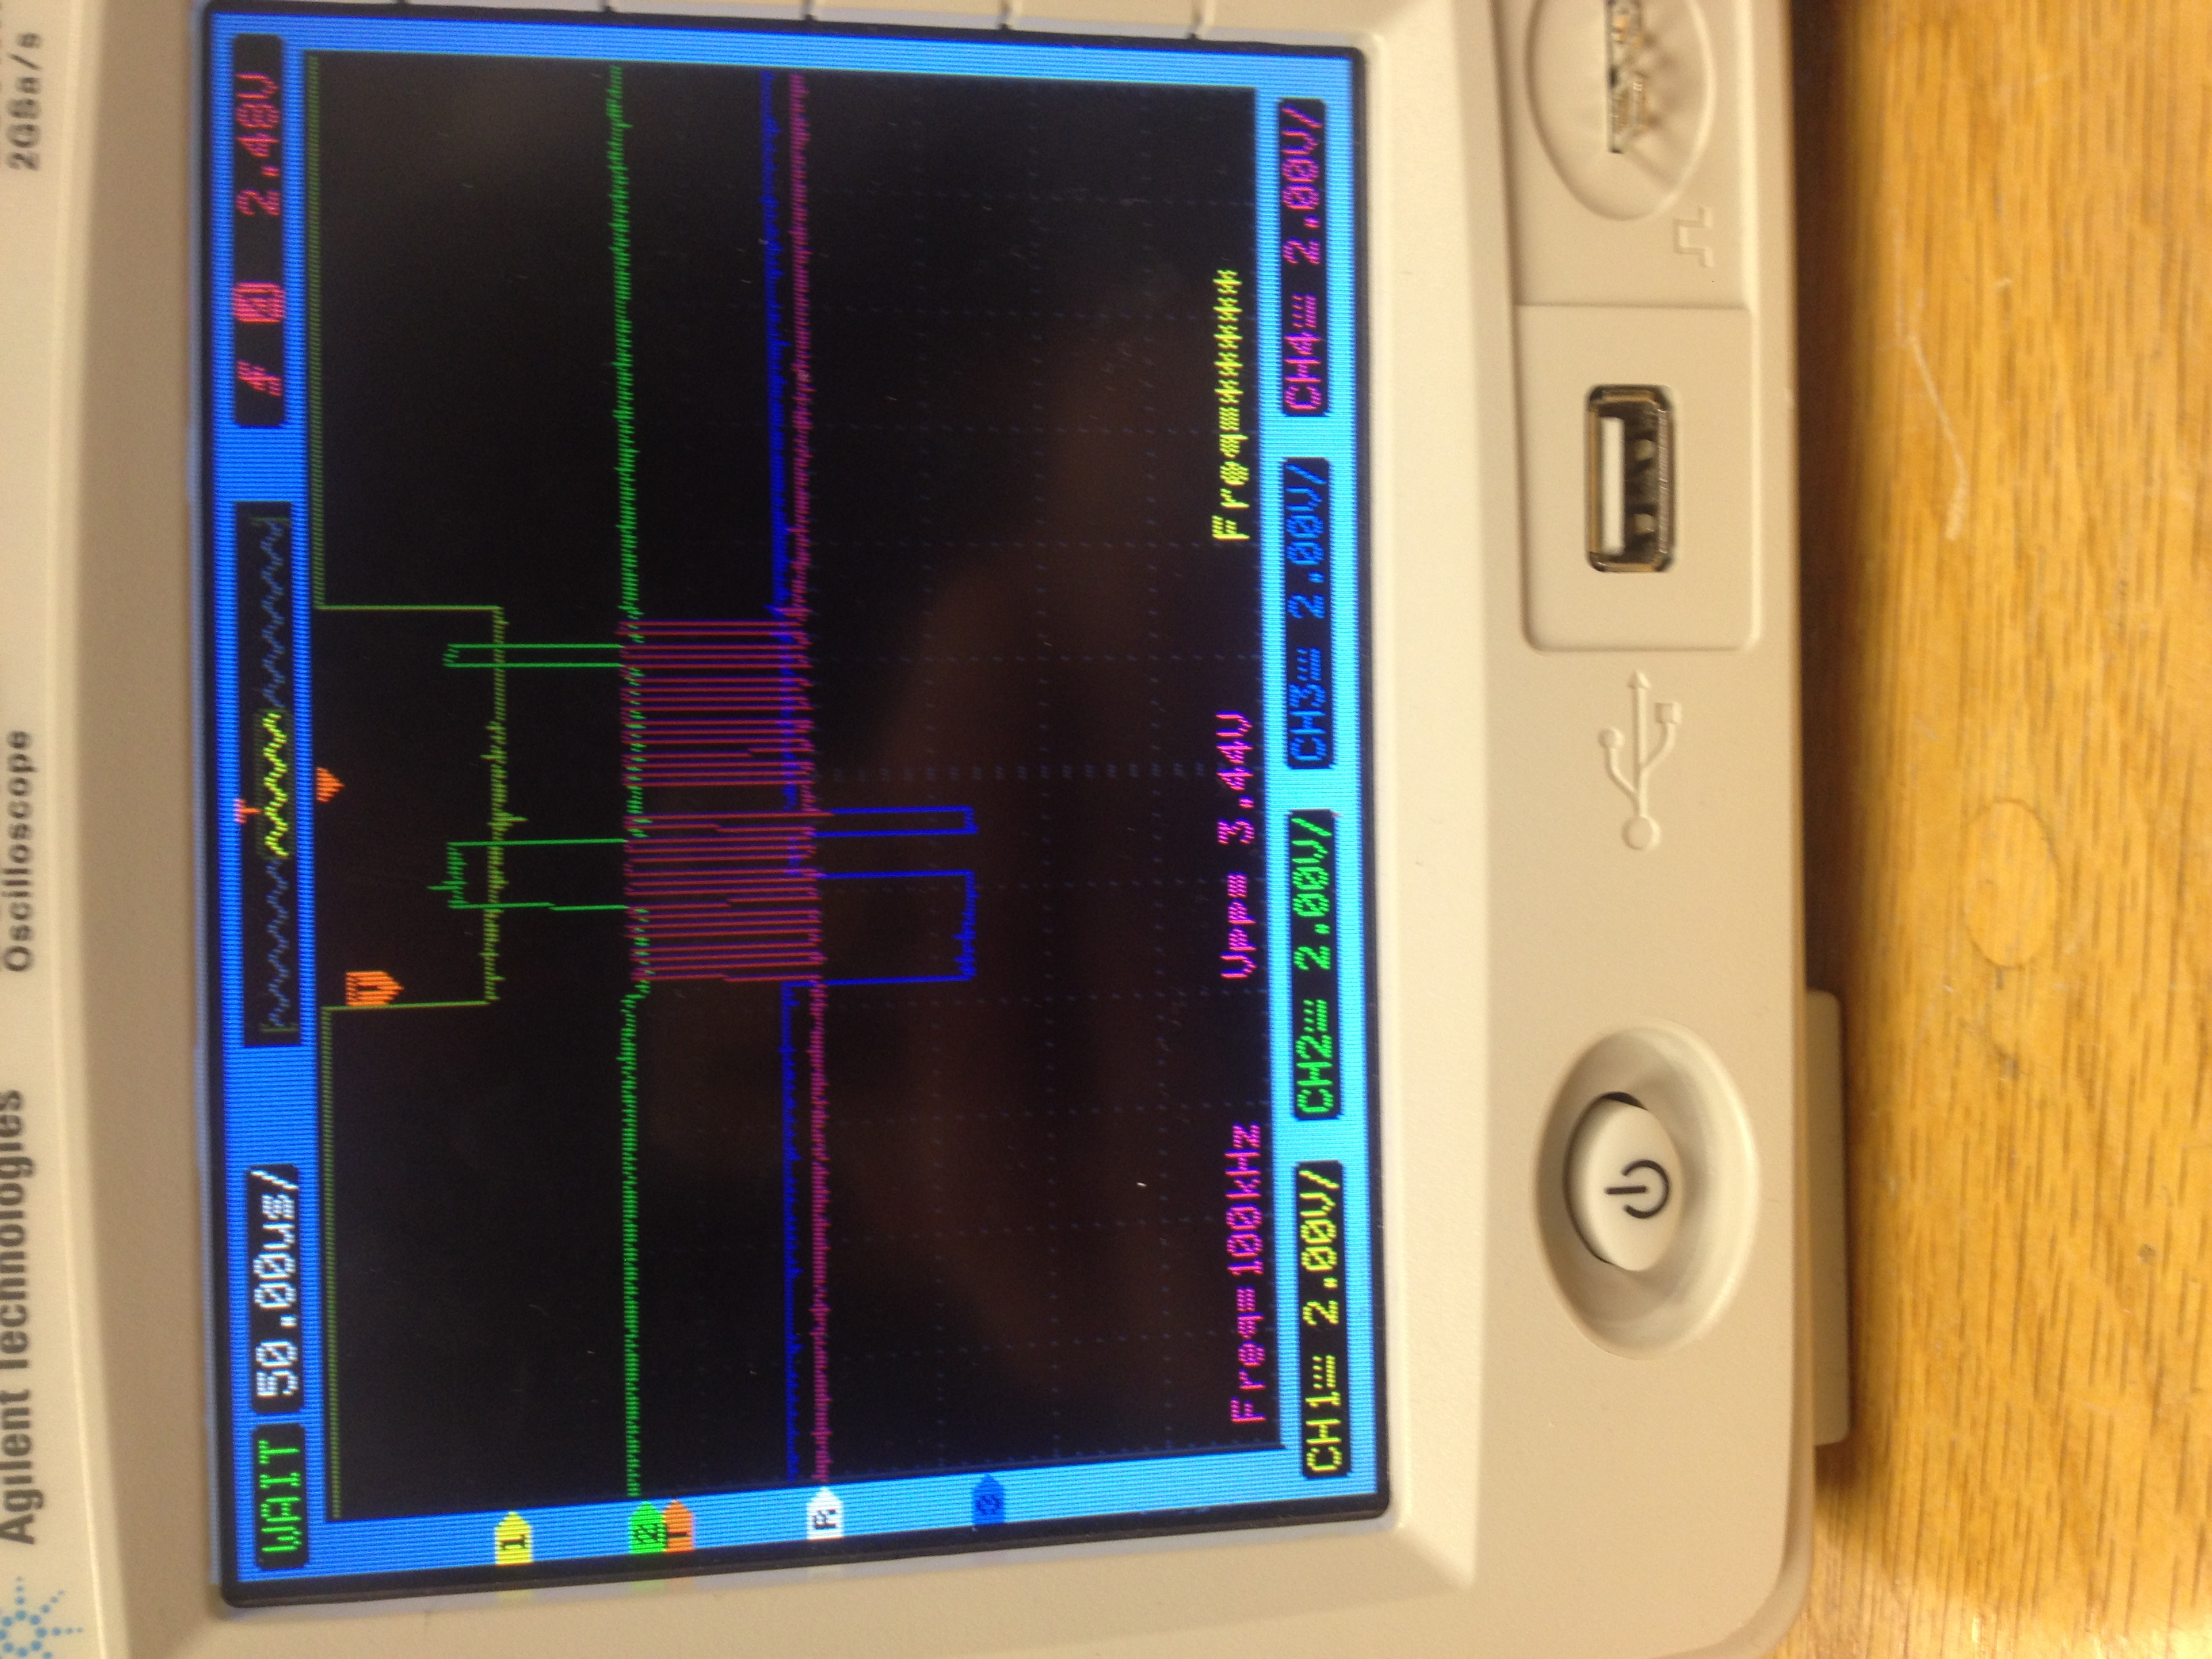
\includegraphics[width=0.6\textwidth,angle=-90]{pwr_config_read.jpg}
    \caption{Reading from the RF configuration register to make sure we are outputting power correctly}
\end{figure}

\begin{figure}[H]
    \centering
    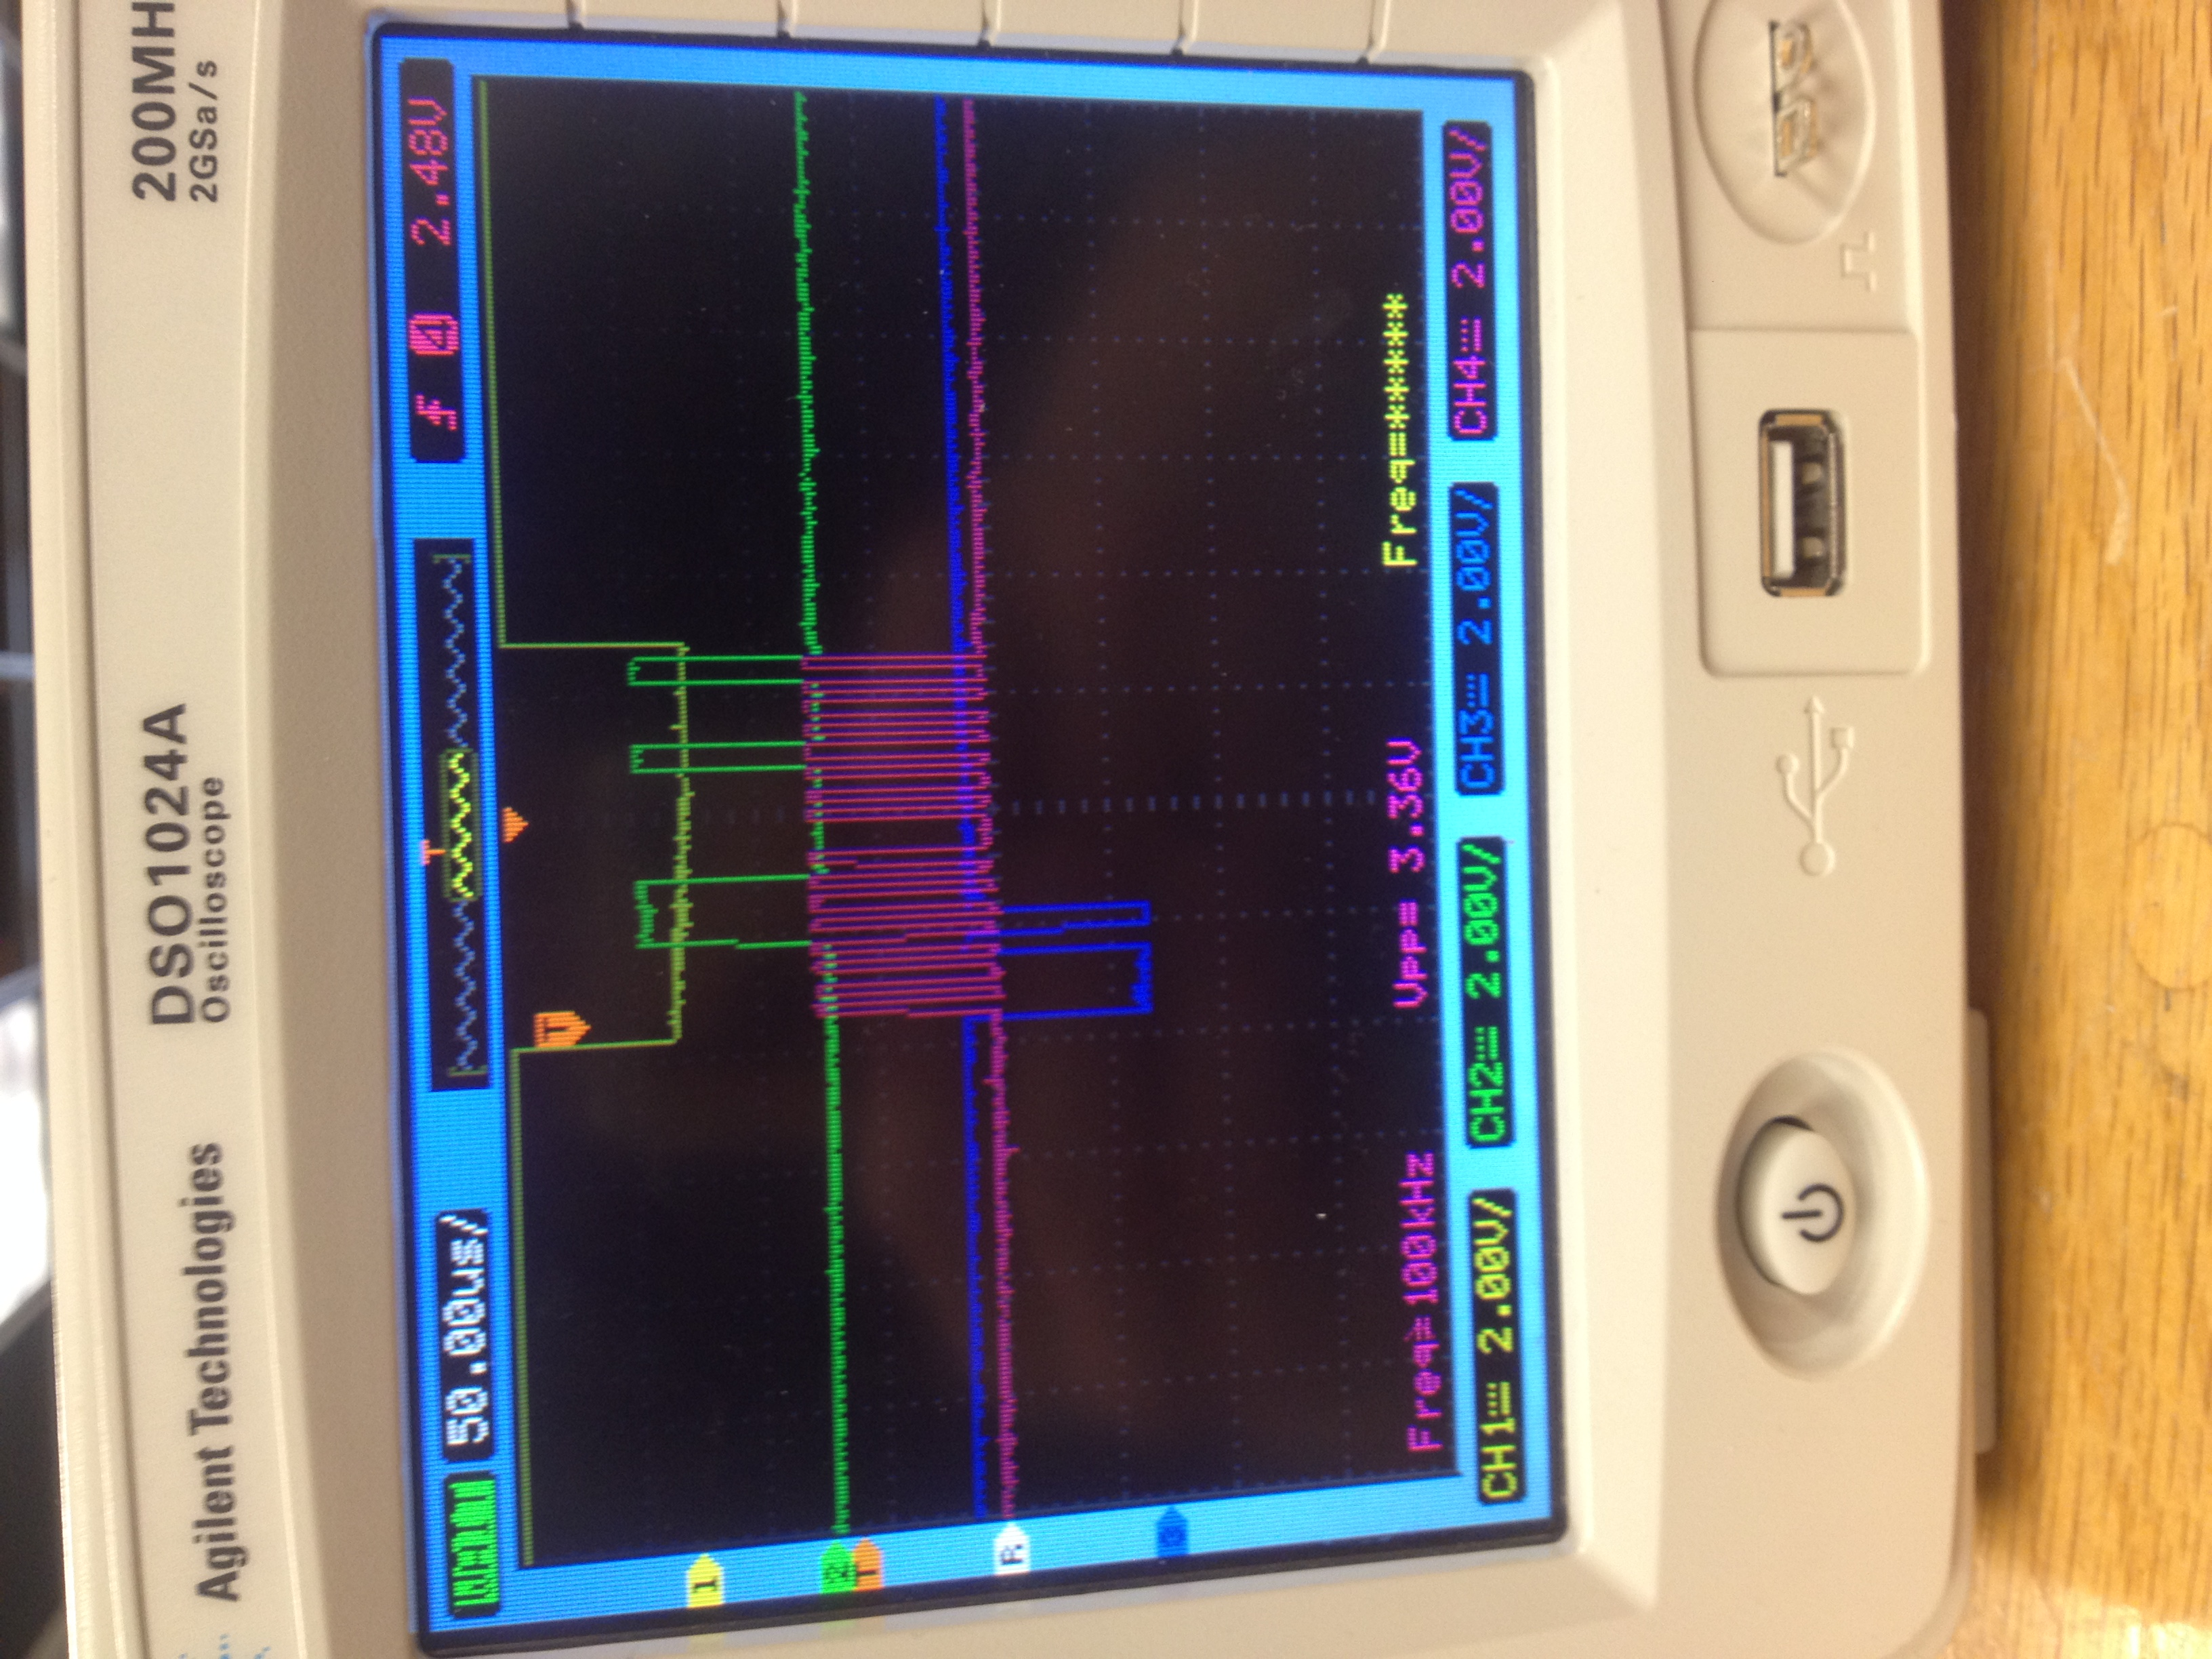
\includegraphics[width=0.6\textwidth,angle=-90]{fifo_status_read.jpg}
    \caption{Reading the FIFO status register}
\end{figure}

\begin{figure}[H]
    \centering
    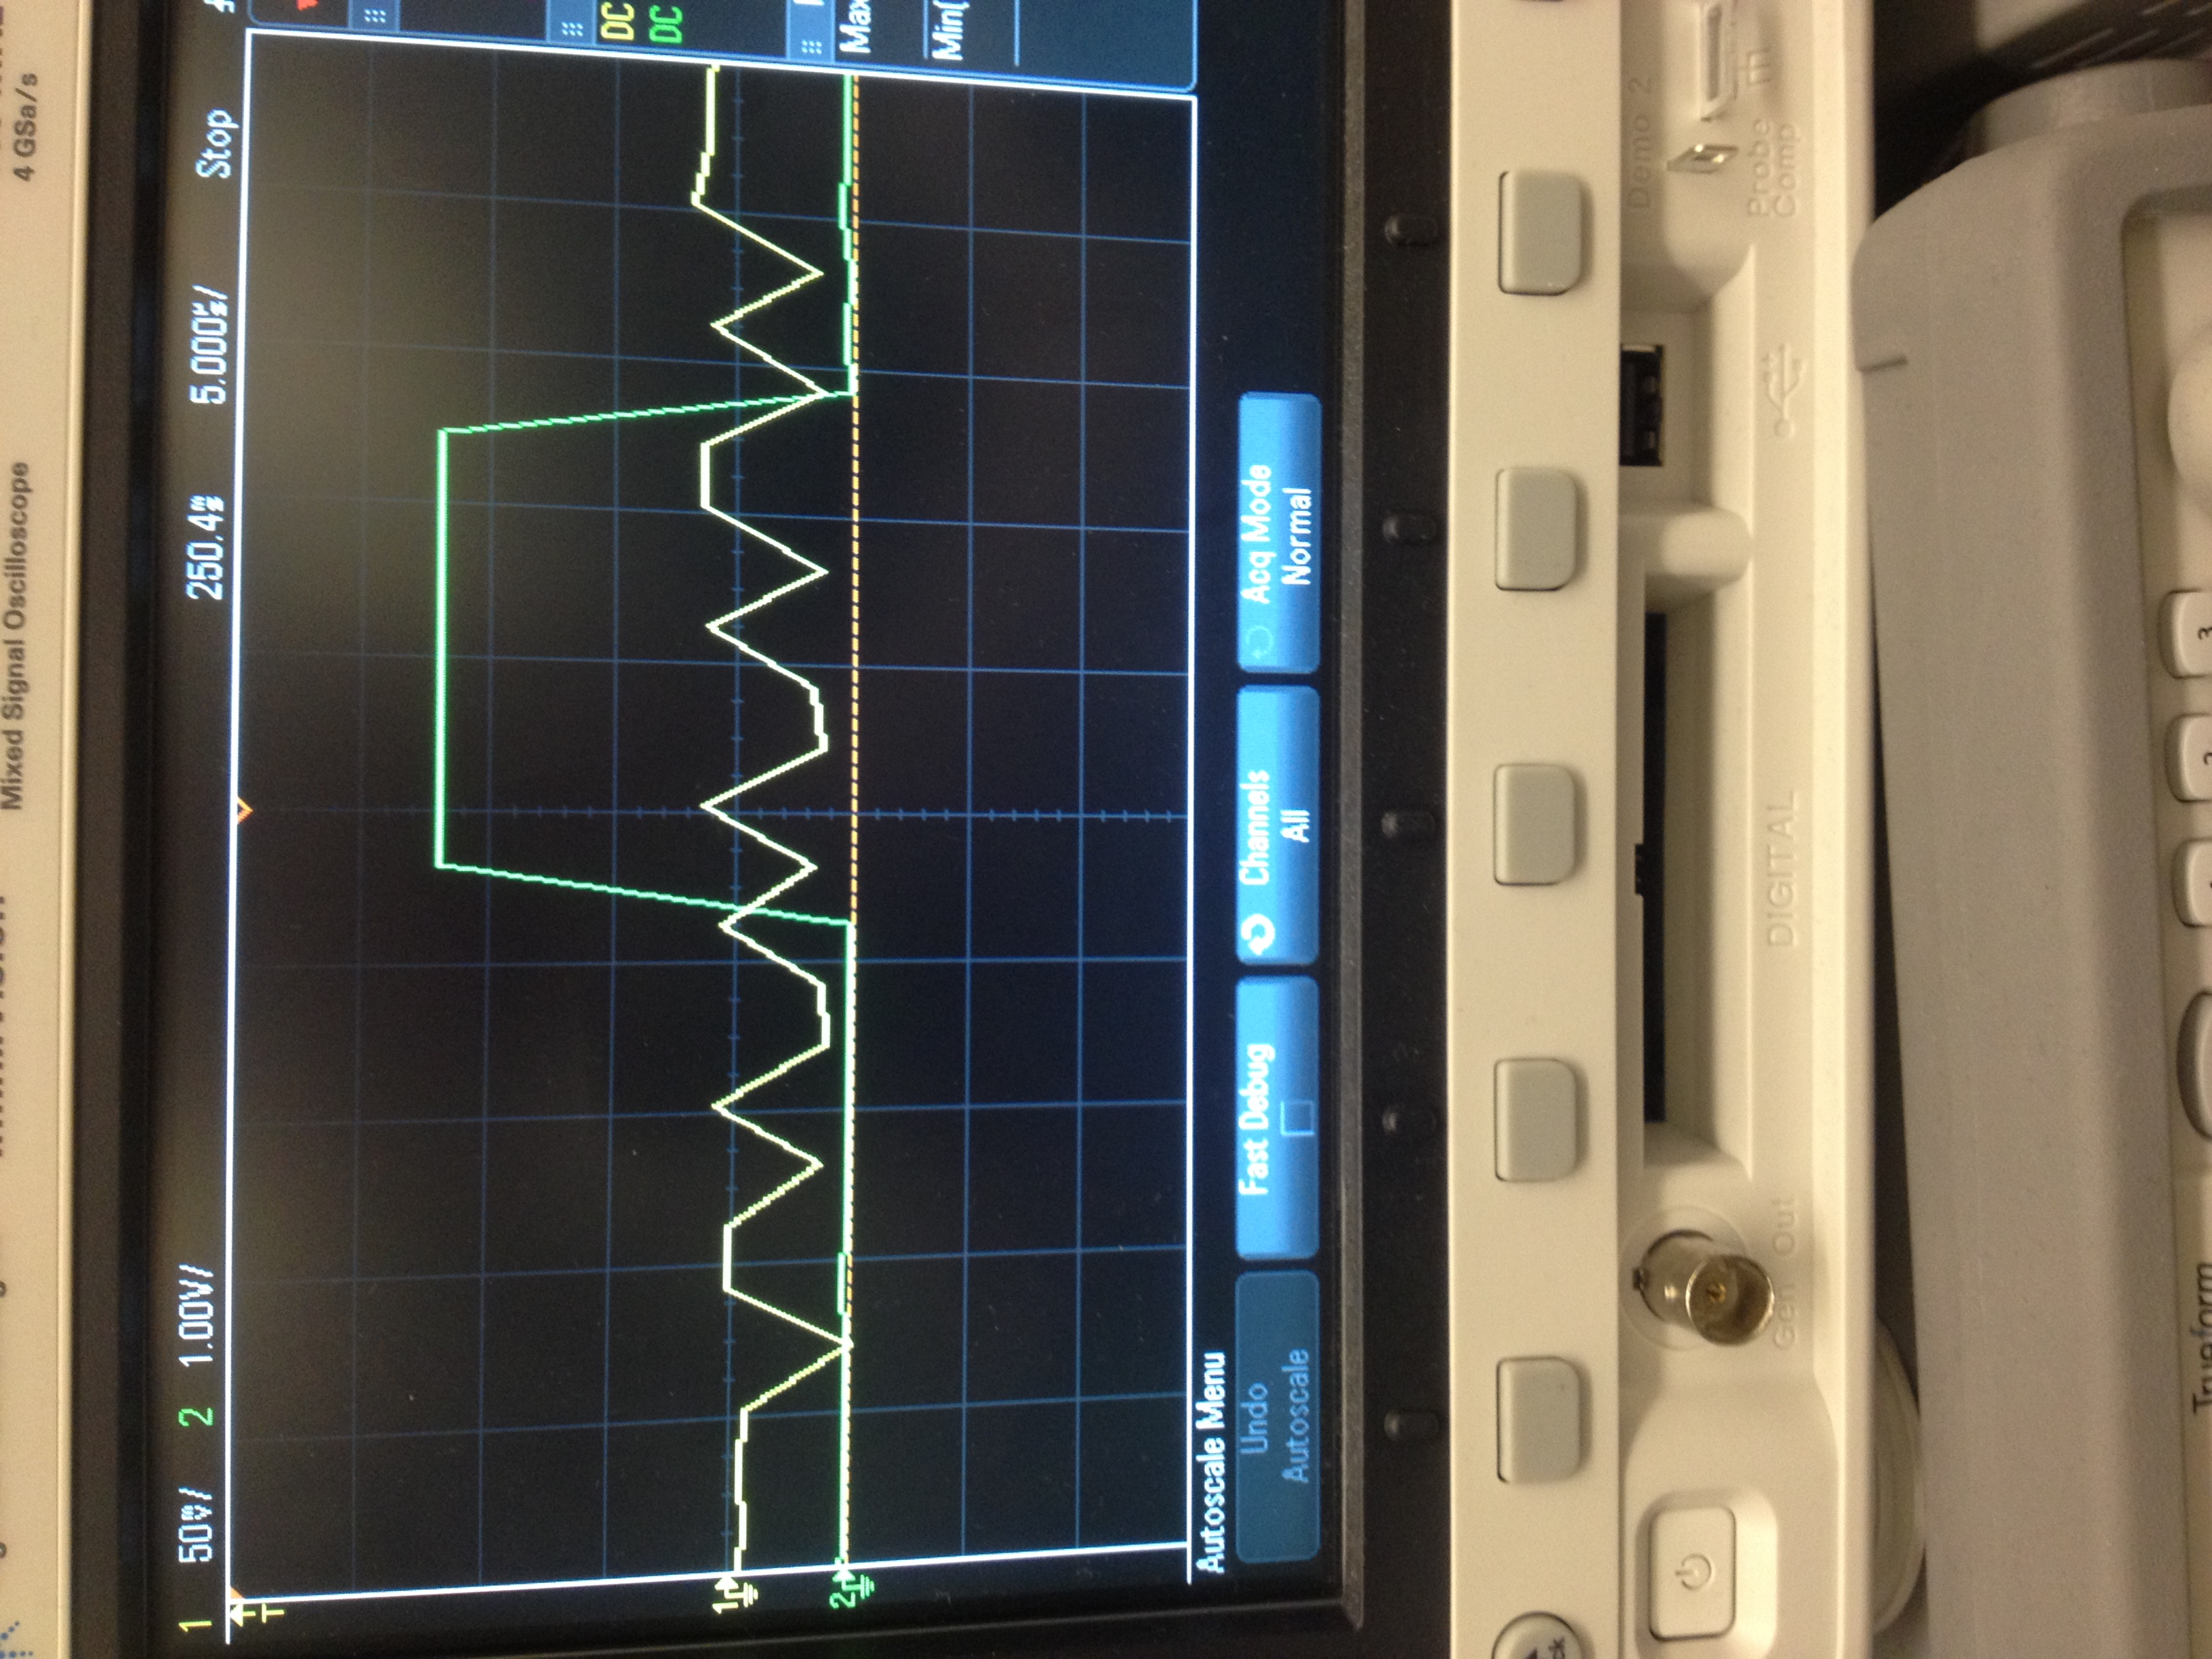
\includegraphics[width=0.6\textwidth,angle=-90]{BEAGLE_FAIL.jpg}
    \caption{The beaglebone being bad at sending SPI signals, note how it is off by one bit.}
\end{figure}

\subsection*{Part 2: Streaming Transceiver Data}
In part 2, the goal was to stream data over the transceiver modules. Despite us being able to write a payload to the transceiver, as well as toggle the chip enable, we were unable to show that we were transmitting data. We were unsure if this was because the buffer didn't flush automatically or because it was not being told to enable properly. Thus the farthest we got on the project was the two screenshots below for the freedom board because again we couldn't get the BeagleBone to send data
over SPI properly.

\begin{figure}[H]
    \centering
    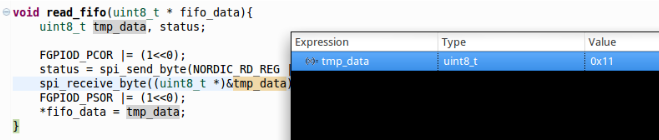
\includegraphics[width=0.7\textwidth]{tx_fifo_flush.png}
    \caption{Before we write a payload to the transceiver we knew it was important to flush the transciever.}
\end{figure}

\begin{figure}[H]
    \centering
    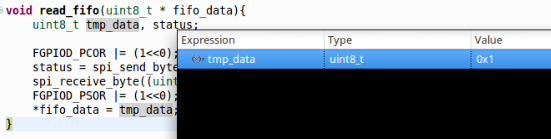
\includegraphics[width=0.7\textwidth]{tx_payload_add.png}
    \caption{As can be seen in the figure, we were able to write a payload to the transceiver transmit buffer.}
\end{figure}

This image shows how one could write firmware and software to implement communication over the SPI module. Obviously this image is not how we did it, but it is a good way to do it. If we had some time and motivation we would probably implement it this way.
\begin{figure}[H]
    \centering
    \includegraphics[width=0.7\textwidth]{ECEN5013_PR4.png}
    \caption{How an ideal implementation of this would be. Implement a Class that automatically sets up the SPI interface. That class has methods that could send an arbitrary amount of data, or read in an arbitrary amount of data. This is done by wrapping the low level firmware calls that access individual bytes from the SPI interface, which is of course implemented in hardware and connected to the Nordic module.}
\end{figure}

\subsection*{Part 3: Wireless Control}
\begin{lstlisting}
asm("nop");
\end{lstlisting}

If we were to implement a structure for sending and receiving commands, it would be implemented similar to an instruction set architecture. 32 bits split up into 5 command bits, instructions on what data to operate on, possibly more command bits, possibly an immediate value. That or just one simple command signal of a byte followed by the proper data to operate on.

\section*{Conclusion}
In this project we have explored software abstraction and SPI implementations for communication. We started by implementing SPI libraries for the freedom board as well as a nordic library that used said freedom SPI libraries and the BeagleBone's already implemented SPI libraries. This didn't work out so well and we failed to make serious inroads into part 2, but Zach has other things due tomorrow and James is off to Japan so we don't have more time to work on it. We both really enjoyed having you as a professor. Really appreciative of your hard work and desire to perfect the class for students. Keep it up and we are sure you will have more fans in the future.
%\captionsetup{labelformat=empty}
\end{document}
